\documentclass[dvipdfmx,11pt]{beamer}
%\graphicspath{{fig_tab/os_presentation/20201215/}}
\usepackage{lipsum}
\usetheme{Verona}
\usepackage{bxdpx-beamer}
\usepackage{pxjahyper}
\usepackage{minijs}
\usepackage{mathpazo}
\usepackage{amsmath,amssymb}
\usepackage{graphicx}
\usepackage{array}
\usepackage{tikz}
\usepackage{wrapfig}
\usepackage{float}
\usepackage{here}
\usepackage{lscape}
\usepackage{ascmac}
\usepackage{tabularx}
\renewcommand{\kanjifamilydefault}{\gtdefault}
\hypersetup{% hyperrefオプションリスト
 setpagesize=false,
 bookmarksnumbered=true,%
 bookmarksopen=true,%
 colorlinks=true,%
 linkcolor=blue,
 citecolor=blue,
 urlcolor = magenta
}
\setbeamertemplate{navigation symbols}{}

\title[Calderon, Fouka, and Tabellini (2022)]{Racial Diversity and Racial Policy Preferences: \\
The Great Migration and Civil Rights}
\subtitle{Calderon, Fouka, and Tabellini (2022)}
\author{Reviewed by Reio TANJI}
\date[6/12/2022 OS Seminar]{July 12th, 2022 \\ Ohtake-Sasaki Seminar}
\institute[]{Osaka University, Graduate School of Economics}

\begin{document}

\begin{frame}\frametitle{}
\titlepage
\end{frame}

\begin{frame}{Abstract}
  \begin{itemize}
    \item Research Question: Is the Great Migration is causally linked with support for civil rights?
    \begin{itemize}
      \item Between 1940 and 1970, more than 4 million African Americans moved from the South to the North of the US.
      \item At the same period witnessed the struggle and eventual success of the civil rights movements.
    \end{itemize}
    \item The (Second) Great Migration: Shift-share IV of Black inflows
    \begin{itemize}
      \item raised support for the Democratic Party
      \item increased Congress members' propensity to promote civil rights legislation
      \item encouraged pro-civil rights activism outside the US South
    \end{itemize} 
  \end{itemize}
\end{frame}

\frame{\tableofcontents}

\section{Introduction}
\frame{\sectionpage}

\begin{frame}{Literature}
  \begin{itemize}
    \item The effect of the inflow of Black voters is puzzling.
    \begin{itemize}
      \item may have shifted northern politicians incentives to introduce civil rights legislation.
      \begin{itemize}
        \item African Americans were largely disenfranchised in the South but faced no voting restrictions in the North
        \item Black population might have also expanded the organizational capacity of the Black civil rights movement (McAdam, 1982)
      \end{itemize}
      \item may have generated political opposition among northern whites
      \begin{itemize}
        \item racial diversity often triggers backlash among members of the majority group (Alesina, Baqir and Easterly, 1999; Enos, 2016; Dustmann, Vasiljeva and Damm, 2019).
      \end{itemize}
    \end{itemize}
    \item in Economic Literature: 
    \begin{itemize}
      \item the Great Migration increased residential segregation (Boustan, 2010)
      \item lowered the economic and social mobility of African Americans in the long run (Derenoncourt, 2022).
    \end{itemize}
  \end{itemize}
\end{frame}

\begin{frame}{}
  \begin{figure}
    \centering
    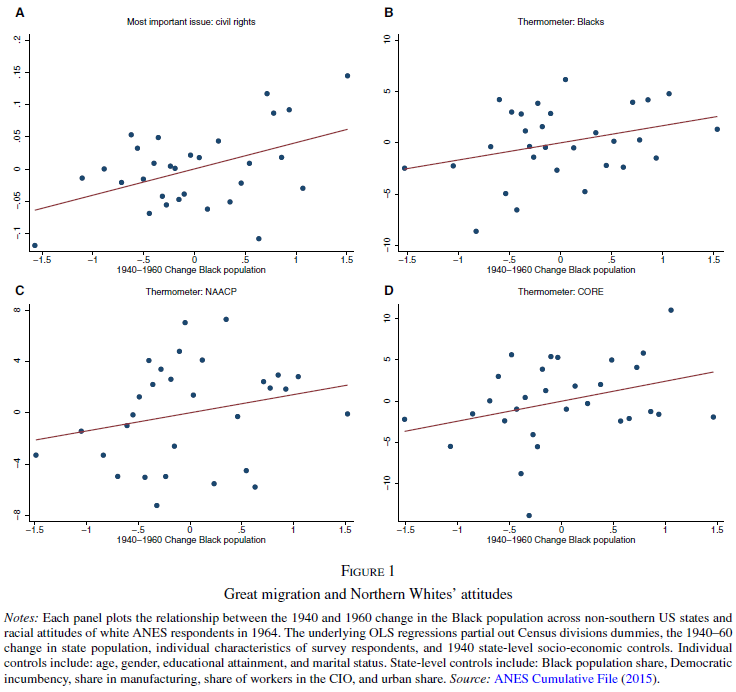
\includegraphics[scale = .45]{fig_tab/os20220708/F1.png}
  \end{figure}
\end{frame}

\begin{frame}{Research Design}
  \begin{itemize}
    \item This article shows a causal relationship between the Black inflow to northern counties (the Great Migration between 1940-1970) and support for civil rights.
    \begin{itemize}
      \item Potentially endogenous migration: Balcks may have migrated to the counties that shows more support for civil rights.
      \item Shift-share instrument (Card, 2001; Boustan, 2010): the expected number of the Black inflow conditional on the preexisting settlements before 1940.
    \end{itemize}
    \item Using the %Data
  \end{itemize}
\end{frame}

\begin{frame}{Summary of Results}
  \begin{itemize}
    \item Black in-migration had a strong, positive impact on the Democratic vote share in Congressional elections.
    \begin{itemize}
      \item 1 ppt increase in the Black population share raised the Democratic vote share by 1.8 percentage points (4\% relative to the 1940 mean).
      \item did not lead to white out-migration or to changes in the composition of white residents at the county level.
    \end{itemize}
    \item Congressional Districts that received more African Americans were represented by legislators with a more
    liberal ideology on racial issues.
  \end{itemize}
\end{frame}

\begin{frame}{Mechanisms}
  \begin{itemize}
    \item the direct effect of Black voters alone is not enough to explain the increase in the Democratic vote share caused by the Great Migration.
    \begin{enumerate}
      \item the changed composition of the electorate (Schickler, 2016; Grant, 2020).
      \item local activism (McAdam, 1982; Biondi, 2021).
    \end{enumerate}
    \item Their dataset shows that approximately 7 white voters would have to switch to the Democratic Party for every 10 Black migrants.
  \end{itemize}
\end{frame}

\begin{frame}{Contribution}
  
\end{frame}

\section{Historical Background}
\frame{\sectionpage}

\section{Data}
\frame{\sectionpage}

\section{Empirical Strategy}
\frame{\sectionpage}

\section{Main Results}
\frame{\sectionpage}

\section{Mechanisms}
\frame{\sectionpage}

\section{Conclusions}
\frame{\sectionpage}

\end{document}
